In this chapter, we develop a Fortran90 \BoxLib\ code to solve the heat equation,
\begin{equation}
\frac{\partial\phi}{\partial t} = \nabla^2 \phi; \quad \phi(t=0) = e^{-100r^2},
\end{equation}
on a domain from [-1,1] in each spatial direction, where $r$ is the distance
to the point $(x,y,z) = (0.5,0.5,0.5)$.  We will
assume that $\Delta x = \Delta y = \Delta z$.  We begin with a simple single-level, 
forward Euler discretization and work up to
a full AMR code with many bells and whistles.  Below is an outline of how we will 
proceed.  Each of these sections contains an accompanying tutoral directory.
\begin{itemize}

\item In Section \ref{Sec:OpenMP}, we develop a single-level code similar to the
{\tt WaveEquation\_F} example in Chapter \ref{Chap:Getting Started}, but add 
support for OpenMP.

\item In Section \ref{Sec:Boundary Conditions} we develop the capability to handle
other (non-periodic) boundary condition types.

\item In Section \ref{Sec:Refinement} we develop the capabilitly to have multiple
levels of refinement using a fixed, multilevel grid structure.

\item In Section \ref{Sec:AMR} we develop the capability to adaptively change the
refined grid structure.

\item In Section \ref{Sec:Linear Solvers} we develop the capability to solve the
equation implicitly, using the linear solver libraries.

\item In Section \ref{Sec:Checkpoints} we develop the capability to write and read
checkpoints for restarting simulations.

\end{itemize}
The basic time-advancement strategy uses the following temporal discretization:
\begin{equation}
\frac{\phi_{ij}^{n+1} - \phi_{ij}^n}{\Delta t} = \left[\nabla\cdot(\nabla\phi)\right]_{ij}.
\end{equation}
In the explicit case, we first compute $\nabla\phi$, at faces using:
\begin{equation}
(\nabla\phi)_{i+\myhalf,j} = \frac{\phi_{i+1,j}^n-\phi_{ij}^n}{\Delta x}.
\end{equation}
We will refer to these face-centered gradients as ``fluxes''.
Next, we compute the update by taking the divergence of these fluxes,
\begin{equation}
\left[\nabla\cdot(\nabla\phi)\right]_{ij} = \frac{(\nabla\phi)_{i+\myhalf,j}-(\nabla\phi)_{i-\myhalf,j}}{\Delta x} + \frac{(\nabla\phi)_{i,j+\myhalf}-(\nabla\phi)_{i,j-\myhalf}}{\Delta y}.
\end{equation}
We use a flux divergence formulation because it will enable a more natural 
extension to multiple levels of refinement, where we will be concerned with
conservation across levels.  Note that in this explicit case, since $\Delta x = \Delta y$, 
the Laplacian reduces to the standard five point stencil two dimensions
(seven point stencil in three dimensions).  

\section{OpenMP}\label{Sec:OpenMP}

A hybrid MPI/OpenMP version of the algorithm described above sits in 
{\tt BoxLib/Tutorials/HeatEquation\_EX1\_F/}.  It is very similar to the
{\tt WaveEquation\_F} example in Chapter \ref{Chap:Getting Started}, so we shall
only highlight some key additional features.

Since the fluxes live on face centers, we need face-centered \MultiFab\ s, i.e.,
\MultiFab\ s that are nodal in one spatial direction.  In {\tt advance.f90},
we build them as follows:
\begin{lstlisting}[backgroundcolor=\color{light-green}]
! an array of multifabs; one for each direction
type(multifab) :: flux(phi%dim) 

! used to build face-centered multifabs
logical :: nodal(phi%dim) 

! build the flux(:) multifabs
do i=1,dm
   nodal(:) = .false.
   nodal(i) = .true.
   ! flux(i) has one component, zero ghost cells, and is nodal in direction i
   call multifab_build(flux(i),phi%la,1,0,nodal)
end do
\end{lstlisting}

To ``thread'' the code, we simply add OpenMP directives (using the {\tt !\$omp parallel do} construct) to any i/j/k loops
we are interested in threading:
\begin{lstlisting}[backgroundcolor=\color{light-green}]
subroutine init_phi_2d(phi, ng, lo, hi, prob_lo, dx)

  integer          :: lo(2), hi(2), ng
  double precision :: phi(lo(1)-ng:,lo(2)-ng:)
  double precision :: prob_lo(2)
  double precision :: dx
 
  ! local varables
  integer          :: i,j
  double precision :: x,y,r2

  !$omp parallel do private(i,j,x,y,r2)
  do j=lo(2),hi(2)
       y = prob_lo(2) + (dble(j)+0.5d0) * dx
       do i=lo(1),hi(1)
          x = prob_lo(1) + (dble(i)+0.5d0) * dx

          r2 = (x*x + y*y) / 0.01
          phi(i,j) = exp(-r2)

       end do
    end do
    !$omp end parallel do

end subroutine init_phi_2d
\end{lstlisting}
This User's Guide is not a manual on OpenMP, so simply note that this particular 
construct tells each thread to work on different values of {\tt j}, with each 
thread getting its own local copy of {\tt i}, {\tt x}, {\tt y}, and {\tt r2}.

Finally, to tell the compiler that we would like to run with OpenMP, we make sure to
set {\tt OMP=t} in the {\tt GNUmakefile}.  Note that you must have you 
{\tt OMP\_NUM\_THREADS} environment variable set properly in order for threads to work.
Also, note that you can enable/disable MPI independently from the OMP flag.  Finally,
here is a sample hopper script (tcsh) for a hybrid MPI/OpenMP job:
\lstinputlisting[backgroundcolor=\color{light-red}]{./AdvancedTopics/hopper_omp.run}
\begin{itemize}
\item ``mppwidth'': how many total cores requested
\item ``-n'': total number of MPI tasks
\item ``-N'': number of MPI tasks per hopper node
\item ``-S'': number of MPI tasks per NUMA node
\item ``-ss'': demands strict memory containment per NUMA node
\item ``-d'': number of OpenMP threads per MPI task
\end{itemize}
\section{Boundary Conditions}\label{Sec:Boundary Conditions}
In order to understand how to implement boundary conditions, we shall 
first describe the general principles behind working with boundary conditions.
The {\tt BoxLib/Tutorials/HeatEquation\_EX2\_F/} tutorial continues our heat
equation example, but now with some non-periodic boundary condition support.  The boundary
condition modules in {\tt BoxLib/Src/F\_BaseLib/} can be used as a springboard
for developing your own customized boundary conditions.

The basic idea is that every grid has knowledge of the
boundary condition type at the low and high side edge in each direction.
Common boundary condition types are {\tt INFLOW}, {\tt OUTFLOW}, {\tt SLIP\_WALL},
{\tt NO\_SLIP\_WALL}, and {\tt PERIODIC}.
There is also an {\tt INTERIOR} boundary condition type, which 
will be explained below.  We use an integer mapping, e.g., {\tt INFLOW}=1,
{\tt OUTFLOW=2}, etc., that is listed in {\tt BoxLib/Src/F\_BaseLib/bc.f90}.
Consider grid 1 in Figure \ref{fig:bc_example1}.  The
low-x boundary condition is {\tt INFLOW}, and the high-y boundary condition is
{\tt NO\_SLIP\_WALL}.  The high-x and low-y boundary conditions are {\tt INTERIOR}, which
means that the ghost cells share the same physical space as cells in the valid region of 
another grid.  Note that for grids 6, 7, 10, and 11, the boundary condition type for
every side is {\tt INTERIOR}.
%%%%%%%%%%%%%%%%%%%%%%%%%%%%%%%%%%%%%
\begin{figure}[tb]
\centering
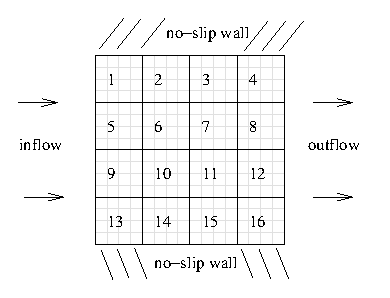
\includegraphics[width=4in]{./AdvancedTopics/bc_example1}
\caption{\label{fig:bc_example1}Two-dimensional example with 16 - 4$^2$grids with
{\tt INFLOW}, {\tt OUTFLOW}, and {\tt NO\_SLIP\_WALL} boundary conditions.
The numbers refer to the grid number.}
\end{figure}
%%%%%%%%%%%%%%%%%%%%%%%%%%%%%%%%%%%%%

Figure \ref{fig:bc_example2} demonstrates a problem with periodicity in the x-direction.
In this case, the low-x boundary condition for grid 1 is {\tt PERIODIC}.  Note there are some
similarities between {\tt PERIODIC} and {\tt INTERIOR} boundary conditions when
it comes to filling ghost cells in that ghost cell values are simply copied in from the valid
region of another grid.  In fact, one can think of {\tt PERIODIC} as just
a special type of {\tt INTERIOR} boundary condition.
For the other boundary conditions types, the user can write custom boundary 
conditions routines to fill ghost cells, which can involve setting ghost cell values 
directly, or using interior points and/or physical boundary conditions in some stencil operation.
%%%%%%%%%%%%%%%%%%%%%%%%%%%%%%%%%%%%%
\begin{figure}[tb]
\centering
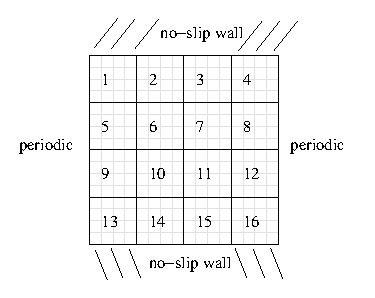
\includegraphics[width=4in]{./AdvancedTopics/bc_example2}
\caption{\label{fig:bc_example2}Two-dimensional example with 16 - 4$^2$grids with
{\tt PERIODIC} and {\tt NO\_SLIP\_WALL} boundary conditions.
The numbers refer to the grid number.}
\end{figure}
%%%%%%%%%%%%%%%%%%%%%%%%%%%%%%%%%%%%%

Now, consider an example with refined grids.  Figure \ref{fig:bc_example3}
contains three grids at the next level of refinement.  In this case, for grid 1,
all of the boundary condition types are {\tt INTERIOR}, even though the neighboring
valid region data is at a coarser level of refinement.  For grid 2, the low-y
boundary condition is {\tt NO\_SLIP\_WALL}, and the low-x, high-x, and hi-y
boundary condition types are {\tt INTERIOR}.
%%%%%%%%%%%%%%%%%%%%%%%%%%%%%%%%%%%%%
\begin{figure}[tb]
\centering
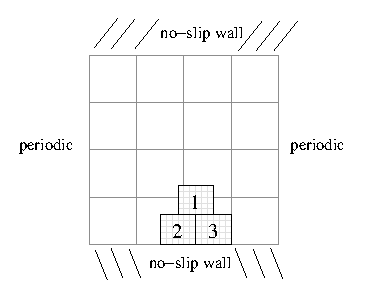
\includegraphics[width=4in]{./AdvancedTopics/bc_example3}
\caption{\label{fig:bc_example3}Two-dimensional example with 3 grids at a finer
resolution than the base grid.}
\end{figure}
%%%%%%%%%%%%%%%%%%%%%%%%%%%%%%%%%%%%%

\section{Multiple Levels of Refinement}\label{Sec:Refinement}
\section{Adaptive Mesh Refinement}\label{Sec:AMR}
\section{Linear Solvers}\label{Sec:Linear Solvers}
\section{Checkpoints and Restarting}\label{Sec:Checkpoints}


